\documentclass{report}
\usepackage{ucs} 
\usepackage[utf8x]{inputenc} 	
\usepackage[czech]{babel}
\usepackage{pdfpages}
\usepackage{graphicx}
\usepackage{hyperref}
\usepackage{graphicx}
\usepackage{datetime}
\usepackage{titlesec}
\usepackage{interval}

\graphicspath{ {./Schematics/} }
\newcommand*\wildcard[2][5cm]{\vspace*{2cm}\parbox{#1}{\hrulefill\par#2}}  

\title{TuxMan - FPGA}
\titleformat{\paragraph}
\date{11/4/2019}
\author{Martin Přívozník}

\begin{document}
  \includepdf[page={1}]{Front-Page}
  \newpage
  \pagenumbering{gobble}

 \section*{Anotace (Resumé)}
 Tématem práce je návrh arkádové hry na RTL úrovni a její implementace na programovatelném hradlovém poli, tj. FPGA. Uživatelský vstup je zajištěn pomocí PS/2 klávesnice a výstup prostřednictvím VGA. K implementaci je použit jazyk VHDL.

\section*{Klíčová slova}
RTL, programovatelné hradlové pole, FPGA, PS/2, VGA, VHDL

 \section*{Summary}
 The topic of this thesis is designing an arcade game on an RTL level and its implementation on a programmable gate array, i.e. FPGA. User input is provided by PS/2 keyboard and output is shown using VGA. Language called VHDL is used for implementation.

\section*{Keywords}
RTL, programmable gate array, FPGA, PS/2, VGA, VHDL

 \newpage
\vspace*{\fill}

 \section*{Čestné prohlášení}
 Prohlašuji, že jsem předkládanou maturitní/ročníkovou práci vypracoval sám a uvedl jsem veškerou použitou literaturu a bibliografické citace.

\vspace{ 2cm}
  V Liberci dne \today
  \hspace{2cm}
  \wildcard{Martin Přívozník}

\newpage
\tableofcontents

\newpage
\pagenumbering{arabic}

\chapter*{Úvod}
\addcontentsline{toc}{section}{Úvod}

\chapter{Analýza}
Tato kapitola obsahuje stručný souhrn znalostí a informací potřebných pro následný návrh a implementaci. V sekci~\ref{sec:cislicovynavrh} je vysvětlen číslicový obvod a postup jeho návrhu. V sekci~\ref{sec:fpga} stručně vysvětluji programovatelné hradlové pole a dále vybranou vývojovou desku. Sekce~\ref{sec:rozhrani} se zabývá použitými komunikačními rozhraními, které zajišťují uživatelský vstup a výstup. Na závěr kapitoly, v sekci~\ref{sec:hrapacman} vysvětluji princip a funkčnost hry, jenž je vzorem pro můj návrh.

\section{Číslicový návrh}\label{sec:cislicovynavrh}
V této sekci se věnuji tomu, co je číslicový obvod a jak jej navrhnout jak ve schématu, tak v jazyce popisujícím hardware. V podsekci~\ref{sec:kombinacniobvody} rozeberu logické funkce, prostředky jejich popisu a realizace pomocí logických hradel. Podsekce~\ref{sec:sekvencniobvody}  je zaměřená na návrh sekvenčních obvodů a synchronních sekvenčních automatů (FSM), na což naváže podsekce~\ref{sec:synchronniaasynchronninavrh}, ve které vysvěluji princip hodinových domén a plně sekvenčního návrhu. V podsekci~\ref{sec:jazykvhdl} stručně ukážu, jak převést schéma číslicového obvodu do kódu v jazyce popisujícím hardware (Hardware Description Language, HDL), v mém případě do jazyka Very High Speed Integrated Circuit Hardware Description Language (VHDL).


\subsection{Kombinační obvody}\label{sec:kombinacniobvody}
\subsubsection{Booleovská funkce}
Booleovská funkce je funkce $N$ vstupů a $M$ výstupů nad množinou $\{0, 1\}$. V případě, kdy má funkce více jak jeden výstup, lze ji rozdělit na $M$ funkcí s jedním výstupem. Uvážíme-li Booleovu algebru, platí pro operace sčítání a násobení pravidla uvedená v tabulce~\ref{tab:pravidla}. 
\begin{table}
\centering
\begin{tabular}{ c c c } 
	$a+ b = b + a$ & $a*b = b*a$ & (komutativita) \\
	$a+(b+c) = (a+b) + c$ & $a*(b*c) = (a*b)*c$ & (asociativita) \\
	$a+(b*c) = (a+b) * (a+c)$ & $a*(b+c) = (a*b) + (a*c)$ & (distributivita) \\
	$a+0 = a$ & $a*1 = a$ & (neutralita 0 a 1) \\
	$a + \overline{a} = 1$ & $a * \overline{a} = 0$ & (vlastnosti negace) \\
\end{tabular}
    \caption{Axiomy a vztahy Booleovy algebry.\cite{boole1854investigation}}
    \label{tab:pravidla}
\end{table}
Operace se dvěma vstupními hodnotami nazýváme binární operace. Některé binární operace, přestože často používají stejná značení + a * jako v algebře reálných čísel, mají v Booleově algebře stejnou prioritu a jiný význam (žádná operace nemá přednost)~\cite{kubatova}. Pro logický součet a logický součin platí základní pravidla v tabulce~\ref{tab:pravidlaboolalgebry}.
\begin{table}
\centering
\begin{tabular}{ c c c } 
	de Morgan & $\overline{(a+b)} = \overline{a} * \overline{b}$ & $\overline{(a*b)} = \overline{a} + \overline{b}$ \\
	idempotence & $a + a = a$ & $a * a = a$ \\
\end{tabular}
    \caption{Základní pravidla Booleovy algebry.\cite{kubatova}}
    \label{tab:pravidlaboolalgebry}
\end{table}
Příkladem reprezentace Booleovské funkce je pravdivostní tabulka~\ref{tab:andtable}, kde $in_1$ a $in_2$ jsou vstupní hodnoty a $out$ je výstupní hodnota. 
\begin{table}
\centering
\begin{tabular}{ |c c|c| } 
   	\hline
	$in_1$ & $in_2$ & $out$ \\
	\hline
	$0$ & $0$ & $f(0,0)$ \\
	$0$ & $1$ & $f(0,1)$ \\
	$1$ & $0$ & $f(1,0)$ \\
	$1$ & $1$ & $f(1,1)$ \\
   	\hline
\end{tabular}
    \caption{Pravdivostní tabulka.}
    \label{tab:andtable}
\end{table}
Pravdivostní tabulka obsahuje vždy $N^2$ řádků, aby reprezentovala výstupní hodnotu pro všechny možné kombinace vstupních hodnot. Další možností je Booleovská formule~.\cite{kubatova}. K vyjádření formule a k popisu booleovské funkce používáme nejčastěji základní funkce uvedené v tabulce~\ref{tab:logickefunkce}
\begin{table}
\centering
\begin{tabular}{ |c|c|c| } 
   	\hline
	Název & Pravdivostní tabulka & Formule \\
   	\hline
	AND (logický součin) & \begin{tabular}{ |c c|c| } 
	   	\hline
		$in_1$ & $in_2$ & $out$ \\
	   	\hline
		$0$ & $0$ & $0$ \\
		$0$ & $1$ & $0$ \\
		$1$ & $0$ & $0$ \\
		$1$ & $1$ & $1$ \\
	   	\hline
	\end{tabular} & $out = in_1*in_2$ \\
   	\hline
	NAND (negovaný logický součin) & \begin{tabular}{ |c c|c| } 
	   	\hline
		$in_1$ & $in_2$ & $out$ \\
	   	\hline
		$0$ & $0$ & $1$ \\
		$0$ & $1$ & $1$ \\
		$1$ & $0$ & $1$ \\
		$1$ & $1$ & $0$ \\
	   	\hline
	\end{tabular} & $out = \overline{in_1*in_2}$ \\
	\hline
	OR (logický součet) & \begin{tabular}{ |c c|c| } 
	   	\hline
		$in_1$ & $in_2$ & $out$ \\
	   	\hline
		$0$ & $0$ & $0$ \\
		$0$ & $1$ & $1$ \\
		$1$ & $0$ & $1$ \\
		$1$ & $1$ & $1$ \\
	   	\hline
	\end{tabular} & $out = in_1+in_2$ \\
	\hline
	NOR (negovaný logický součet) & \begin{tabular}{ |c c|c| } 
	   	\hline
		$in_1$ & $in_2$ & $out$ \\
	   	\hline
		$0$ & $0$ & $1$ \\
		$0$ & $1$ & $0$ \\
		$1$ & $0$ & $0$ \\
		$1$ & $1$ & $0$ \\
	   	\hline
	\end{tabular} & $out = \overline{in_1+in_2}$ \\
	\hline
	NOT (logická negace) & \begin{tabular}{ |c|c| } 
	   	\hline
		$in_1$ & $out$ \\
	   	\hline
		$0$ & $1$ \\
		$1$ & $0$\\
	   	\hline
	\end{tabular} & $out = \overline{in_1}$ \\
	\hline
	BUFFER (opakovač) & \begin{tabular}{ |c|c| } 
	   	\hline
		$in_1$ & $out$ \\
	   	\hline
		$0$ & $0$ \\
		$1$ & $1$\\
	   	\hline
	\end{tabular} & $out = in_1$ \\
	\hline
	XOR (nonekvivalence) & \begin{tabular}{ |c c|c| } 
	   	\hline
		$in_1$ & $in_2$ & $out$ \\
	   	\hline
		$0$ & $0$ & $0$ \\
		$0$ & $1$ & $1$ \\
		$1$ & $0$ & $1$ \\
		$1$ & $1$ & $0$ \\
	   	\hline
	\end{tabular} & $out = in_1 \oplus in_2$ \\
	\hline
	XNOR (ekvivalence) & \begin{tabular}{ |c c|c| } 
	   	\hline
		$in_1$ & $in_2$ & $out$ \\
	   	\hline
		$0$ & $0$ & $1$ \\
		$0$ & $1$ & $0$ \\
		$1$ & $0$ & $0$ \\
		$1$ & $1$ & $1$ \\
	   	\hline
	\end{tabular} & $out =\overline{in_1 \oplus in_2}$ \\
   	\hline
\end{tabular}
    \caption{Tabulka nejpoužívanějších základních logických funkcí.}
    \label{tab:logickefunkce}
\end{table}
\subsubsection{Kombinační obvod}
Kombinační logický obvod, je takový obvod, ve kterém jsou výstupní hodnoty dány pouze aktuální kombinací vstupních proměnných. Neobsahuje žádnou paměť předchozích stavů. Jedinou vyjímkou je krátký časový interval, za který logický člen (AND, NAND, OR, NOR ...) vyhodnotí výstup na základě vstupních hodnot. Tento časový interval může být zanedbatelný v případě krátkých datových cest. V případě dlouhé datové cesty může být potřeba na tento časový interval brát zřetel a zvážit optimálnější řešení. \par
Platí, že u číslicových obvodů každá proměnná v operaci nabývá hodnotu jednoho tzv. bitu. Bit je základní jednotkou dat a může nabývat hodnot $0$, nebo $1$. Reprezentací číslicového obvodu je schéma číslicového obvodu, kde každá z funkcí je reprezentována tzv. schématickou značkou. Schématické značky mohou být různé, dokud z nich jasně vyplívá, jakou funkci zastupují. Schématické značky jsou propojené signály, které představují jednotlivé bity. Pro minimalizaci je možné několik signálů (bitů) zakreslit jediným konektorem, pokud je označený počtem bitů, které reprezentuje. Nejčastěji používané normy značení jsou evropská a americká. Příklady schéma\-tických značek pro nejpoužívanější logické funkce jsou uvedené v tabulce~\ref{tab:functionschemes}. 
\begin{table}
\centering
\begin{tabular}{ c c } 
	AND & \raisebox{-0.4\height}{\includegraphics[scale=0.6]{/Gates/AND.png}} \\
	NAND & \raisebox{-0.4\height}{\includegraphics[scale=0.6]{/Gates/NAND.png}} \\
	OR & \raisebox{-0.4\height}{\includegraphics[scale=0.6]{/Gates/OR.png}} \\
	NOR & \raisebox{-0.4\height}{\includegraphics[scale=0.6]{/Gates/NOR.png}} \\
	NOT & \raisebox{-0.4\height}{\includegraphics[scale=0.6]{/Gates/NOT.png}} \\
	BUFFER & \raisebox{-0.4\height}{\includegraphics[scale=0.6]{/Gates/BUFFER.png}} \\
	XOR & \raisebox{-0.4\height}{\includegraphics[scale=0.6]{/Gates/XOR.png}} \\
	XNOR & \raisebox{-0.4\height}{\includegraphics[scale=0.6]{/Gates/XNOR.png}} \\
\end{tabular}
    \caption{Schématické značky některých nejpouživanějších základních logických funkcí (americká norma ANSI).}
    \label{tab:functionschemes}
\end{table}
Pro usnad\-nění práce můžeme využívat logických bloků, které plní danou funkci. Opět platí, že ze značení logických bloků ve schématu musí plně vyplívat, jakou funkci zastupují. Logický blok, který má definovanou funkci může být použit schématu. Při návrhu číslicových obvodů využíváme hierarchie, kde jsou pro každý logický blok popsány vstupy i výstupy a v případě, kdy se nejedná o základní logické bloky, tak je popsána i funkce (formule, pravdivostní tabulka, nebo schéma bloku) a vhodně přiřazena ke schématu. Jedním ze základních logických bloků je poloviční sčítačka, viz obrázek~\ref{fig:halfadder}.
\begin{figure}
\centering
\includegraphics[width=0.9\columnwidth]{/LogicalBlocks/HalfAdder.png}
\caption{Schéma poloviční sčítačky a příklad jejího značení ve schématu.}
\label{fig:halfadder}
\end{figure}
 Poloviční sčítačka umí sečíst dvě jednobitová čísla a vygenerovat bit do vyššího řádu (carry) podle pravdivostní tabulky~\ref{tab:halfaddertab}.
\begin{table}
\centering
 \begin{tabular}{ |c c|c c| } 
   	\hline
	$A$ & $B$ & $C$ & $\sum$ \\
   	\hline
	$0$ & $0$ & $0$ & $0$ \\
	$0$ & $1$ & $0$ & $1$\\
	$1$ & $0$ & $0$ & $1$\\
	$1$ & $1$ & $1$ & $0$\\
   	\hline
\end{tabular}
	\caption{Pravdivostní tabulka poloviční sčítačky.}
	\label{tab:halfaddertab}
\end{table}
Zřetězením dvou polovičních sčítaček a přenesením pomocí funkce OR získáme poté kompletní sčítačku, viz obrázek~\ref{fig:fulladder}.\cite{kubatova}
\begin{figure}
\centering
\includegraphics[width=0.9\columnwidth]{/LogicalBlocks/FullAdder.png}
\caption{Schéma kompletní sčítačky a příklad jejího značení ve schématu.}
\label{fig:fulladder}
\end{figure}
Kompletní sčítačka umí sečíst jednobitová čísla, vygenerovat bit do vyššího řádu a přijmout bit z nižšího, sčítá tedy tři bity. Sčítá počet jedniček na vstupech. \par
Pro porovnávání dvou hodnot a vyhodnocení jejich nerovnosti používáme tzv. komparátor, viz obrázek~\ref{fig:comparator}. 
\begin{figure}
\centering
\includegraphics[width=0.9\columnwidth]{/LogicalBlocks/Comparator.png}
\caption{Schéma komparátoru a příklad jejího značení ve schématu}
\label{fig:comparator}
\end{figure}
Dalším důležitým základním logickým blokem je multiplexor, viz obrázek~\ref{fig:mux}.
\begin{figure}
\centering
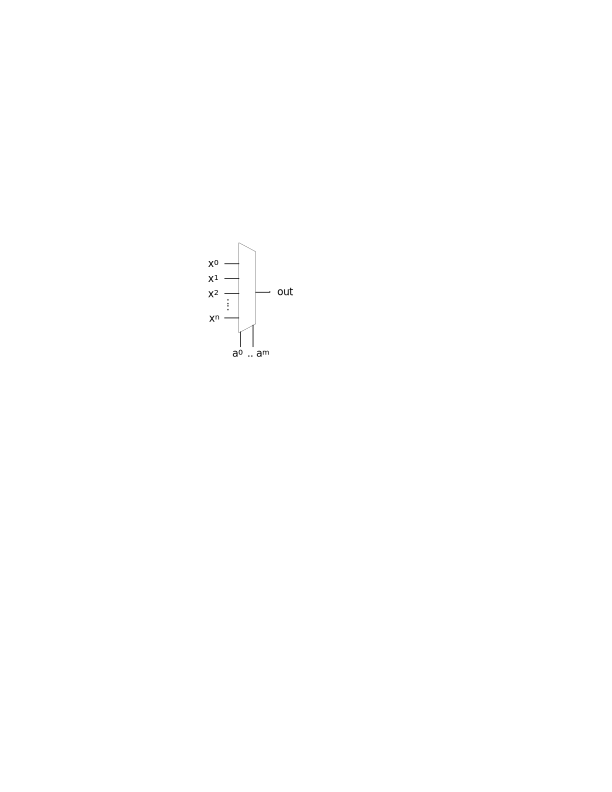
\includegraphics{/LogicalBlocks/Mux.pdf}
\caption{Schématická značka multiplexoru}
\label{fig:mux}
\end{figure}
Multiplexor na základě řídícího vstupu/řídících vstupů ($a$) přivádí na výstup ($out$) jeden ze vstupních signálů ($x$). Číslicový obvod lze realizovat například z integrovaných obvodů, v nichž bývají hradla realizována z několika tranzistorů. Logické hodnoty představuje napětí přivedené na obvod. Logická $1$ bývá reprezentována  napětím vyšším než 3,3 Voltů a logická $0$ napětím nižším.

\subsection{Sekvenční obvody}\label{sec:sekvencniobvody}
\subsection{Synchronní a asynchronní návrh}\label{sec:synchronniaasynchronninavrh}
\subsection{Jazyk VHDL}\label{sec:jazykvhdl}

\section{Programovatelná hradlová pole FPGA}\label{sec:fpga}
Tato sekce se zabývá tím, co jsou programovatelná hradlová pole (Field of programmable gate array, FPGA) a jak probíhá práce s těmito hradlovými poli na vývojové desce. V podsekci~\ref{sec:dostupneprostredky} popisuji části FPGA, které jsou použity pro implementaci číslicového obvodu. Podsekce~\ref{sec:logickasynteza} stručně vysvětluje kroky nezbytné pro implementaci samotného číslicového obvodu na základě jeho popisu VHDL kódem. V podsekcích \ref{sec:basys2} a \ref{sec:xilinxise} je stručně popsána použitá vývojová deska a vývojové prostředí, které se váže k FPGA, které deska obsahuje.

\subsection{Dostupné prostředky}\label{sec:dostupneprostredky}
\subsection{Logická syntéza}\label{sec:logickasynteza}
\subsection{Vývojová deska Digilent Basys 2}\label{sec:basys2}
\subsection{Prostředí Xilinx ISE}\label{sec:xilinxise}

\section{Rozhraní}\label{sec:rozhrani}
Tato sekce popisuje komunikační rozhraní použitá v návrhu a implementaci, která zajišťují uživatelský vstup a výstup. V podsekci~\ref{sec:7segment} vysvětluji rozhraní 7-segmentového displeje. Sekce  \ref{sec:ps2} a \ref{sec:vga} popisují protokoly PS/2 a VGA.
\subsection{7-segmentový displej}\label{sec:7segment}
\subsection{PS/2}\label{sec:ps2}
\subsection{VGA}\label{sec:vga}

\section{Hra Pacman}\label{sec:hrapacman}
Tato sekce vysvětluje hru, již má můj návrh klonovat. Podsekce~\ref{sec:principhry} popisuje cíl a pravidla hry. V podsekci~\ref{sec:ovladanihry} vysvětluji ovládání hry.
\subsection{Princip}\label{sec:principhry}
\subsection{Ovládání}\label{sec:ovladanihry}

\chapter{Návrh hry}
V této kapitole se zabývám návrhem herní logiky, na základě které je navržen číslicový obvod pro finální implementaci. Sekce~\ref{sec:specifikacehry} rozebírá konkrétní prvky hry a návrhy pro jejich řešení. V sekci~\ref{sec:hernitextury} vysvětluji, jak jsou navržené textury, které se zobrazují na výstup.

\section{Specifikace hry}\label{sec:specifikacehry}
V této sekci rozebírám konkrétní prvky hry a vysvětluji návrhy pro jejich řešení. V podsekci~\ref{sec:cilachovani} popisuji, jak má hra fungovat jako celek a jak dosáhnout cíle hry. Podsekce~\ref{sec:mapajakomrizka} vysvětluje návrh herního pole, na kterém se hra odehrává a sekce~\ref{sec:postavyachovani} poté popisuje, jak se chovají jednotlivé postavy na navrženém herním poli.

\subsection{Cíl a chování hry}\label{sec:cilachovani}
\subsection{Herní mapa}\label{sec:mapajakomrizka}
\subsection{Postavy a jejich chování}\label{sec:postavyachovani}

\section{Herní textury}\label{sec:hernitextury}
Tato sekce popisuje návrh textur, které se zobrazují na výstup. V podsekci~\ref{sec:RGB} vysvětluji způsob použití barev pro výstup. Sekce~\ref{sec:texturyjakomatice} se zabývá tím, v jaké podobě jsou textury, které se mají propisovat. 
\subsection{RGB}\label{sec:RGB}
\subsection{Textury jako matice barev}\label{sec:texturyjakomatice}

\chapter{Implementace}
Tato kapitola se zabývá návrhem číslicových obvodů pro jednotlivé logicky oddělené bloky na základě herní logiky a jejich implementací. Sekce \ref{sec:ctenizps2} a \ref{sec:vystupnavga} popisují číslicové obvody navržené pro čtení vstupních dat z klávesnice a generování výstupu na monitor. Sekce~\ref{sec:hernilogika} poté vysvětluje vnitřní zapojení jednotlivých bloků zajišťujících logickou funkčnost hry. V sekci~\ref{sec:celek} je poté popsáno kompletní zapojení všech částí do funkčního celku.

\section{Modul pro čtení z PS/2 klávesnice}\label{sec:ctenizps2}
V této sekci vysvětluji číslicový obvod, který jako celek zpracovává vstupní signál z klávesnice a generuje daný výstup. Podsekce~\ref{sec:zpracovanivstupu} rozebírá číslicový obvod pro zpracování vstupního signálu a podsekce~\ref{sec:generovanivystupu} řeší číslicový obvod pro generování výstupního signálu.
\subsection{Zpracování vstupu}\label{sec:zpracovanivstupu}
\subsection{Generování výstupu}\label{sec:generovanivystupu}

\section{Modul pro výstup na VGA monitor}\label{sec:vystupnavga}
Tato sekce popisuje číslicový obvod, který zařizuje funkčnost monitoru a možnost propsání výstupu na něj. V podsekci~\ref{sec:casovanivga} popisuji obvod, který zajišťuje funkčnost a v podsekci~\ref{sec:propsanitextur} vysvětluji, jak propisuji textury na monitor.
\subsection{Časování VGA}\label{sec:casovanivga}
\subsection{Propsání textur na monitor}\label{sec:propsanitextur}

\section{Herní logika}\label{sec:hernilogika}
V této sekci popisuji číslicový obvod, který zajišťuje vnitřní funkcionalitu samotné hry. V podsekci~\ref{sec:hernimapa} je vysvětlený obvod, který řeší herní plochu, na které se postavy pohybují. Podsekce~\ref{sec:ovladanipostav} popisuje obvod ovládající postavy ve hře a v podsekci~\ref{sec:cilehry} je vysvětlen obvod, který řeší splnění cílů hry.
\subsection{Herní mapa}\label{sec:hernimapa}
\subsection{Ovládání postav}\label{sec:ovladanipostav}
\subsection{Cíle hry}\label{sec:cilehry}

\chapter{Testování}

 \chapter*{Závěr}
 \addcontentsline{toc}{section}{Závěr}

\bibliographystyle{ieeetran}
\bibliography{bibfile}

\end{document}